\documentclass[../../main.tex]{subfiles}

\begin{document}
    Um in den folgenden Kapiteln zeitlich-qualitativ optimierte Ergebnisse aus den Messungen zu erhalten, untersuchen wir das Verhalten des Teleskops SALSA in Abhängigkeit von der Zeitmittelung. Hierzu betrachteten wir bereits am Experimenttag qualitativ die Rauschausprägungen bei $\delta t\in\{\SI{1}{\s},\SI{3}{\s},\SI{10}{\s},\SI{30}{\s},\SI{100}{\s},\SI{300}{\s}\}$ und vergleichen diese untereinander. Dabei schauen wir mit dem Teleskop in Richtung $l = \SI{100}{\degree}$ und $b = \SI{0}{\degree}$ im \emph{switched mode}.
    \begin{figure}[H]
        \centering
        \includegraphics[width=0.8\textwidth]{Bilddateien/Signalanalyse/spectrum_64931_64936.pdf}
        \caption{Vergleich des best- und worst-case Spektrums bei $\delta t = \SI{1}{\s}$ und $\delta t = \SI{300}{\s}$. Dabei meinen wir mit \enquote{rel. velocity} stets die Relativgeschwindigkeit zum \emph{local standard of rest} (LSR), also das Sonnenruhesystem.}
        \label{fig:bestworstcomp}
    \end{figure}
    In Abbildung \ref{fig:bestworstcomp} vergleichen wir den kürzesten und längsten der getesteten Belichtungswerte. Hierbei fällt die zunehmende Glattheit der Spektren auf, was grundsätzlich der Auswertung zugute kommt, jedoch in Randfällen ebenfalls mögliche dicht beieinanderliegende oder miteinander verschränkte Peaks aufweichen lassen könnte. Da wir in der Auswertung unten ebenfalls mit einem Glättungsalgorithmus arbeiten werden, genügen wir uns der in der Versuchsanleitung \cite{doc:SALSAStudentManual} angegebenen Zeit von $\delta t = \SI{60}{\s}$, welche wir in Abbildung \ref{fig:nexttime100} mit unserem nächstgemessenen Wert vergleichen.
    \begin{figure}[H]
        \centering
        \includegraphics[width=0.8\textwidth]{Bilddateien/Signalanalyse/spectrum_64935.pdf}
        \caption{Nächster Vergleichswert zu unser tatsächlich gewählten Belichtungszeit von $\delta t = \SI{60}{\s}$.}
        \label{fig:nexttime100}
    \end{figure}
    Aus Interesse schalten wir in einer weiteren Messung den Messmodus des Teleskops von \emph{switched} auf \emph{signal} um und erhalten das in Abbildung \ref{fig:signalmode} dargestellte Spektrum. Hierbei fällt auf, dass die Peaks im Vergleich zu Abbildung \ref{fig:nexttime100} in einem deutlichen Hintergrundsignal verschoben sind und drastisch an Eigenauflösung eingebüßt haben. Den Berg des Hintergrundsignals erklären wir uns durch optisch-geometrische Beugungen und Interferenzen innerhalb der Teleskopschüssel. Insgesamt ist das so erhaltene Signal nicht zur Auswertung geeignet und wir bleiben bei unserem gewählten Messmodus \enquote{\emph{switched}}.

    \begin{figure}[H]
        \centering
        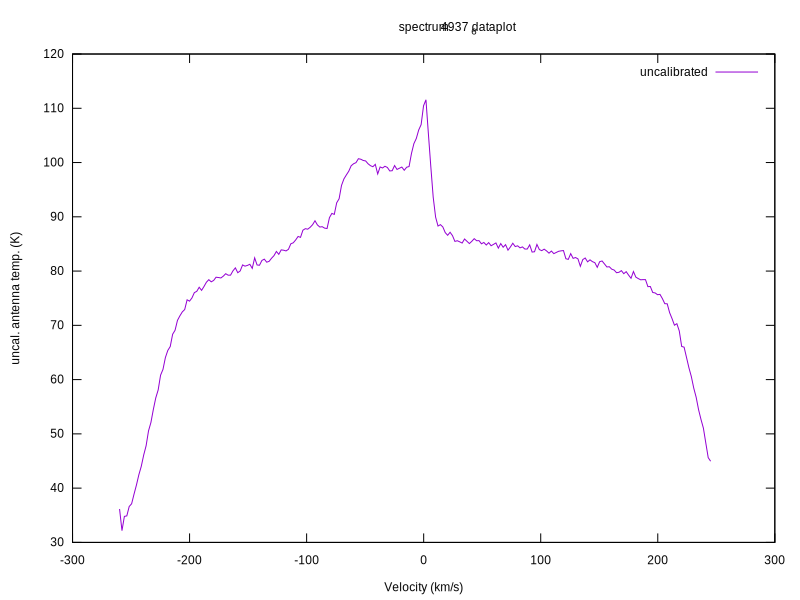
\includegraphics[width=0.8\textwidth]{Bilddateien/Signalanalyse/spectrum_64937.pdf}
        \caption{Spektrum bei $\delta t = \SI{100}{\s}$ im \emph{signal mode}.}
        \label{fig:signalmode}
    \end{figure}
    
\end{document}